\chapter{Лабораторная работа №8 \\
\Large Исследование динамических свойств радиоэлектронных средств при ударном возбуждении}

Цель работы: изучение требований к измерительному тракту при действии ударных импульсных нагрузок, исследование динамических свойств высокочастотного акселерометра и функциональной ячейки (ФЯ) радиоэлектронных средств (РЭС).

Оборудование: ударный стенд \ref{fig:shock-bench}, источник питания, ЛИПС~П-30, анализатор спектра СК~4\==56.

\begin{figure}[H]
    \centering
    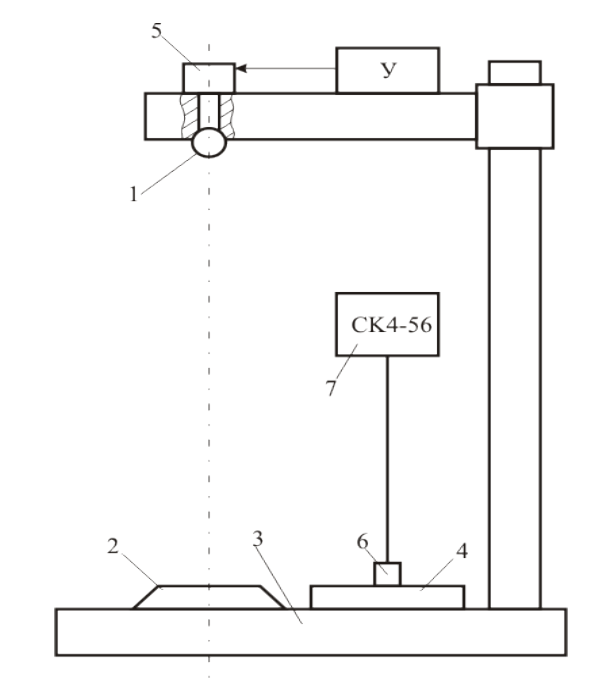
\includegraphics[width=0.5\textwidth]{shock-bench}
    \caption{Схема ударного испытательного стенда:
        1 "--- шар-ударник;
        2 "--- наковальня;
        3 "--- основание стенда;
        4 "--- функциональная ячейка;
        5 "--- механизм сброса ударника;
        6 "--- акселерометр;
        7 "--- анализатор спектра.
    }
    \label{fig:shock-bench}
\end{figure}

\section{Теоретические сведения}

Удар представляет собой импульсные ускорения высоких уровней.
При ударе происходит изменение количества движения за промежуток времени, равный длительности ударного импульса $t$, которое определяется импульсом силы
\[
    F = \int \limits_0^{t+\tau} F(t) dt = m \Delta v,
\]
где $F(t)$ "--- мгновенное значение силы при ударе, $m \Delta v$ "--- изменение количества движения.

Колебания конструкций, вызванные ударом, являются частным случаем случайных вибраций.
Для характеристики одиночных ударов пользуются интегралом Фурье, который представляет собой непрерывную функцию в виде суммы бесконечно большого числа гармонических колебаний, близких по частоте, с бесконечно малыми амплитудами:
\[
    F(t) = \frac{1}{2 \pi} \int \limits_{-\infty}^{\infty} S(\omega) e^{j \omega t} d\omega,
\]
где $S(\omega)$ "--- спектральная плотность воздействия $F(t)$; $\omega$ "--- круговая частота колебаний.

Теоретически ударный импульс содержит энергию во всей полосечастот от нуля до $\infty$.
Для идеального его воспроизведения требуется акселерометр с бесконечной полосой пропускания.
Учитывая, что главная часть энергии ударного импульса содержится в ограниченном диапазоне частот, его характеристики можно зарегистрировать с помощью пьезорезистивных или пьезоэлектрических акселерометров.

Качество измерения параметров удара и динамических характеристик конструкций зависит от формы, амплитуды, длительности ударного импульса, возможностей неискаженного восприятия и передачи спектра удара акселерометром и измерительным трактом.

Совокупность частот, которые могут быть переданы через тракт измерений в обработки сигнала, называют полосой пропускания.
Нижняя и верхняя границы полосы пропускания и коэффициент демпфирования являются важными параметрами акселерометра, влияющими на качество измерений.

Частотные характеристики акселерометров должны удовлетворять следующим условиям.
Для ударов большой длительности целесообразно использовать пьезорезистивные акселерометры, имеющие ненулевую чувствительность в статическом режиме ($\omega_1 = 0$), для ударов малой длительности "--- пьезоэлектрические акселерометры с широкой полосой пропускания и высокой резонансной частотой или пьезорезистивные акселерометры с оптимальным демпфированием $\epsilon = 0.7$, у которых отсутствует отрицательное воздействие фазового сдвига.

Чтобы избежать уменьшения полосы пропускания, необходимо идеальное состояние установочной поверхности и большая жесткость крепления акселерометра.
Чтобы обеспечить правильные фазовые соотношения между частотными составляющими ударного импульса, средства измерений совместно о акселерометром должны иметь равномерную АЧХ в широком частотном диапазоне.

Акселерометр для исследования ударных воздействий рекомендуется выбирать с учетом следующих соотношений:
\[
    f_{0А} \phi \ge 30,
\]
где $f_{0А}$ "--- собственная частота колебаний акселерометра,
\[
    f_{0А} \ge \frac{1}{Т_0},
\]
где $\phi$ "--- длительность фронта ударного импульса; $T_0$ "--- период собственных колебаний массы акселерометра $m_{A}$.

Таким образом, частота собственных колебаний акселерометра, полоса пропускания регистрирующей аппаратуры и длительность ударного импульса "--- основные факторы, определяющие достоверность результатов измерений.

Акселерометр можно представить как систему с одной степенью свободы, состоящую из инерционной массы $m_A$, упругого элемента жёсткостью $k$ и демпфера с коэффициентом затухания $h$ (рис. \ref{fig:accelerometer-oscillation-system}).
Такая колебательная модель описывается уравнением
\begin{equation}\label{eq:oscillation-model-equation}
    z'' + 2 h z' + \omega_{0А}^2 z = f(t),
\end{equation}
где $\omega_{0А} = \sqrt \frac{k}{m_А}$ "--- круговая частота собственных колебаний акселерометра; $m_A$, $k$ "--- инерционная масса и жёсткость акселерометра; $f(t)$ "--- закон измеряемого ускорения.
Решение уравнения \eqref{eq:oscillation-model-equation} имеет вид
\begin{equation}\label{eq:solve-of-oscillation-model-equation}
    z(t) = \frac{g^{k(t)}}{\omega_{0А}^2} - \frac{g}{\omega_{0А}^2} e^{-h t} \int \limits_0^t \left(e^{-h t} k (\tau)\right)' \cos \omega_{0А} (t - \tau) d\tau,
\end{equation}
где $k(t)$ "--- функция перегрузки, $k(t) = \frac{f(t)}{g}$; для синусоидального импульса $k(t) = k_{\max} \sin \frac{\pi t}{2 \tau}$ (рис. \ref{fig:sinusoidal-shock-impulse}), для треугольного импульса $k(t) = k_{\max} \frac{t}{\tau \phi}$.

\begin{figure}[H]
    \centering
    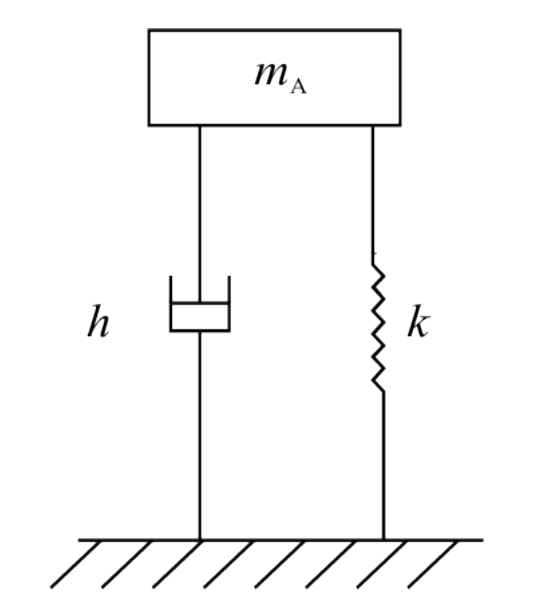
\includegraphics[width=0.5\textwidth]{accelerometer-oscillation-system}
    \caption{Колебательная система акселерометра.}
    \label{fig:accelerometer-oscillation-system}
\end{figure}

\begin{figure}[H]
    \centering
    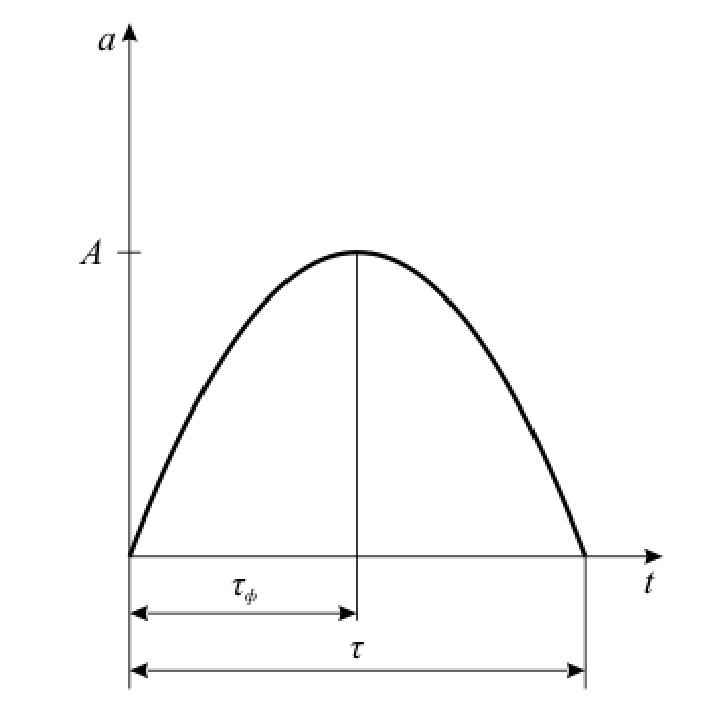
\includegraphics[width=0.5\textwidth]{sinusoidal-shock-impulse}
    \caption{Синусоидальный ударный импульс.}
    \label{fig:sinusoidal-shock-impulse}
\end{figure}

Первое слагаемое уравнения \eqref{eq:solve-of-oscillation-model-equation} характеризует статическое перемещение инерционной массы акселерометра, которое определяет величину выходного сигнала, второе слагаемое "--- динамическую составляющую перемещений, которая определяет погрешность измерений.

При отсутствии затухания в системе акселерометра ($h = 0$) максимальная величина динамического перемещения может быть определена по формуле
\[
    z_{Д \max} = \frac{g}{\omega_0^2} \cdot \frac{T_0}{2 \tau_{ф}}.
\]

При условии $Т_0 << \tau_{ф}$ динамической составляющей перемещения можно пренебречь.
Относительная погрешность акселерометра можетбыть определена по выражению
\begin{equation}\label{eq:relative-error}
    \eta = \frac{z_{Д \max}}{z_{ст}} = \frac{1}{2 f_{0А} k_{\max} \tau_{ф}},
\end{equation}
где $z_{ст} = g k(t) / \omega_{0А}^2$; $k_{\max} = 10$.

Для исследования динамических свойств конструкций РЭС используют ударные стенды, в которых воздействие возникает за счёт взаимодействия ударника и наковальни.
Ударный импульс характеризуется следующими параметрами: аплитудой ускорения $A$; длительностью $\tau$ и условной круговой частотой
\begin{equation}\label{eq:angular-frequency}
    \omega = \pi / \tau~[с^{-1}].
\end{equation}

Коэффициент передачи удара для полусинусоидального импульсавычисляют по выражению
\begin{equation}
    k_{y} = \frac{2 \upsilon}{\upsilon^2 - 1} \cos \frac{\pi}{2 \upsilon},
\end{equation}
где $\upsilon = \omega / \omega_0$ "--- коэффициент расстройки; $\omega_0$ "--- круговая частота собственных колебаний ФЯ РЭС.

Максимальное ускорение и перемещение, воздействующее на испытуемую конструкцию ФЯ, находим по формулам
\begin{align}
    z_{\max} = A k_{у}; \\
    z_{\max} = A k_{у} / \omega_0^2 \ge z = 0.003 a, \label{eq:max-displacement}
\end{align}
где $a$ "--- длина ФЯ.

О характере деформаций элементов конструкций ФЯ при колебаниях можно судить по виду форм (рис. \ref{fig:oscillation-forms}).
Форма является графической иллюстрацией колебательного процесса и отображает положение конструкции в момент наибольшего удаления от положения равновесия.
Первый резонанс является ''зонтичной'' формой колебаний, при которой деформации имеют один знак, а узловые линии отсутствуют, второй резонанс "--- ''крутильной'' формой.
\begin{figure}[H]
    \centering
    \begin{subfigure}[b]{0.45\textwidth}
        \centering
        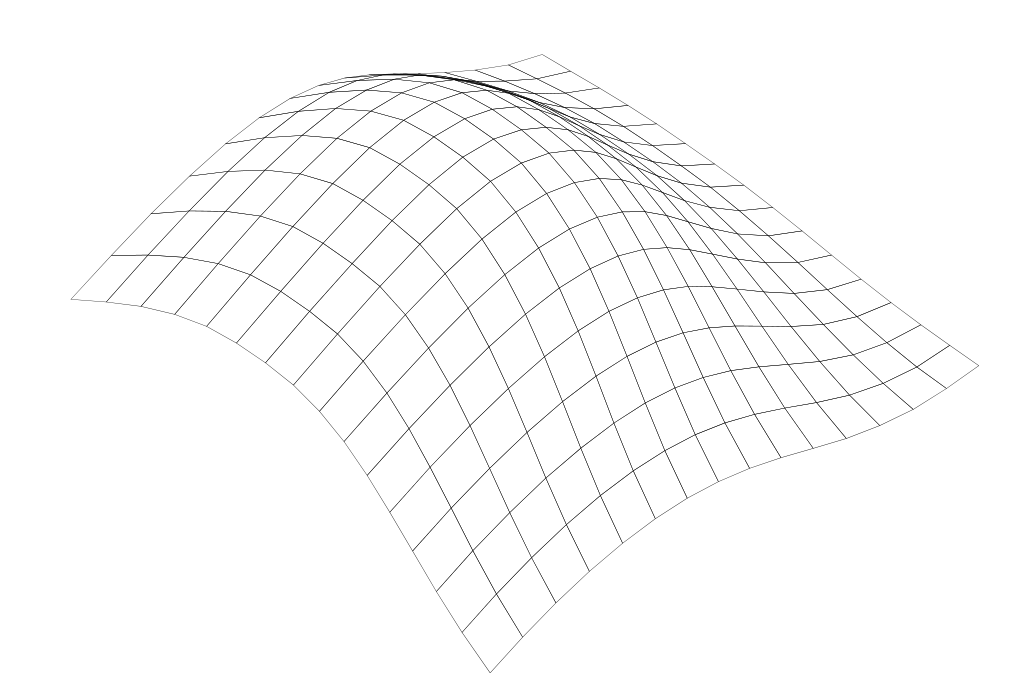
\includegraphics[width=\textwidth]{first-oscillation-form}
        \caption{}
        \label{fig:first-oscillation-form}
    \end{subfigure}
    \hfill
    \begin{subfigure}[b]{0.45\textwidth}
        \centering
        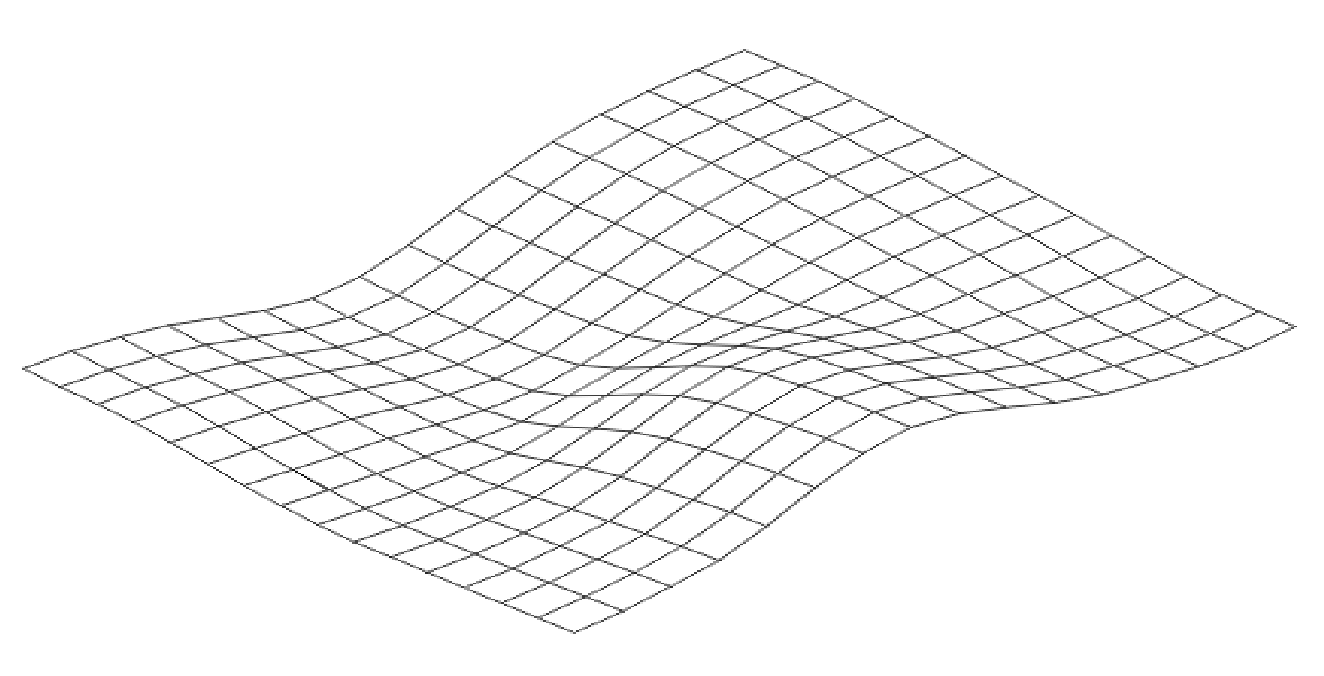
\includegraphics[width=\textwidth]{second-oscillation-form}
        \caption{}
        \label{fig:second-oscillation-form}
    \end{subfigure}
    \caption{Собственные формы колебаний ФЯ:
        а "--- первая;
        б "--- вторая.
    }
    \label{fig:oscillation-forms}
\end{figure}

Первую собственную круговую частоту ФЯ определяют поформуле
\[
    \omega_0 = \frac{\alpha}{a^2} \sqrt \frac{D a b}{m},
\]
где $\alpha$ "--- коэффициент, зависящий от способа закрепления; $m$ "--- масса ФЯ; $D = \frac{E h^3 (1 - \mu^2)}{12}$ "--- цилиндрическая жёсткость; $b$, $h$ "--- ширина итолщина ФЯ; $Е$, $\mu$ "--- приведённый модуль упругости и коэффициент Пуассона материала ФЯ.

Для ФЯ, закрепленной в четырех точках, с учётом $f_0 = \omega_0 / 2 \pi$ и массы акселерометра $M$, расположенной в центре, частоту собственных колебаний в Герцах определяют как
\begin{equation}\label{eq:normal-mode}
    f_0 = \frac{\pi}{2 a^2} \left(1 + \frac{a^2}{b^2}\right) \sqrt \frac{D a b}{m (1 + 44 M / m)}.
\end{equation}

\begin{comment}
1. Опытным путём определю частоту $f_0$ собственных колебаний ячейки РЭС в Герцах и коэффициент передачи удара в диапазоне частот $(0.8\==1.2) f_0$.

2. Расчётным путём определю статическую, динамическую деформацию и относительную погрешность измерений акселерометра и динамические характеристики ячейки РЭС при ударном возбуждении.
\end{comment}

Характеристики акселерометра:
\begin{itemize}
    \item полоса пропускания $\Delta f = (20\==10000)~Гц$;
    \item собственная частота колебаний $f_{0А}30000~Гц$;
    \item масса акселерометра $M 3.3~г$.
\end{itemize}


Характеристики ФЯ:
\begin{itemize}
    \item приведённый модуль упругости $E = ГПа$;
    \item коэффициент Пуассона $\mu = 0.3$;
    \item плотность материала ячейки $p = 1.85~г/м^3$.
    \item масса ячейки $m = 15.1~г$.
    \item размер ячейки $a \times b \times h = 95 \times 78 \times 1.0~мм$.
\end{itemize}

Характеристики полусинусоидального ударного импульса:
\begin{itemize}
    \item амплитуда ускорения $A = 100~м/с^2$;
    \item длительность $\tau = 2~мс$;
    \item длительность фронта нарастания нагрузки $\tau_{ф} = 1~мс$;
\end{itemize}

\section{Выполнение работы}

1. Определю частоту $f_0$ собственных колебаний ячейки РЭС по формуле \eqref{eq:normal-mode}.

2. Определю выходной сигнал акселерометра, установленного в месте крепления ФЯ $A_{кр}$ и геометрическом центра $A_{ц}$ ячейки РЭС при ударном возбуждении в диапазоне частот $(0.8\==1.2) f_0$.
Результаты опытов занесу в таблицу \ref{tab:dynamic-parameters}.

\begin{table}[H]
    \centering
    \caption{Динамические свойства ФЯ РЭС}
    \label{tab:dynamic-parameters}
    \begin{tabular}{|c|c|c|c|c|c|c|c|}
        \hline
        \multirow{2}{*}{Параметры} & \multicolumn{7}{c|}{$f,~Гц$}            \\ \cline{2-8} 
                                   & 240 & 260 & 280 & 300 & 320 & 340 & 360 \\ \hline
        $A_{кр}$                   &     &     &     &     &     &     &     \\ \hline
        $A_{ц}$                    &     &     &     &     &     &     &     \\ \hline
        $k_{у}$                    &     &     &     &     &     &     &     \\ \hline
    \end{tabular}
\end{table}

3. Определю коэффициенты передачи удара ячейки РЭС при ударном возбуждении в диапазоне частот $(0.8\==1.2) f_0$ по формуле
\[
    k_{y} = \frac{A_{ц}}{A_{кр}}.
\]

Результаты расчётов занесу в форму таблицы и построю графическую зависимость $k_{y} = \phi(t)$, где $f$ "--- частота фильтра виброанализатора.
Определю опытное значение частоты собственных колебаний $f_{ОЭ}$ ячейки РЭС.

4. Определю относительную погрешность измерений акселерометра по формуле \eqref{eq:relative-error}.

5. Определю параметры ударного импульса и основныединамические характеристики ячейки РЭС по формулам \eqref{eq:angular-frequency}\==\eqref{eq:max-displacement}.

6. Сравню экспериментальные и расчетные значения динамических свойств ячейки РЭС ($f_0$, $k_{у}$).
